\section{Ejercicio 3.}

Código de la tarea de batch

\begin{Verbatim}[commandchars=\\\{\}]
\PY{k}{const} \PY{k+kt}{char} \PY{n}{bloquea} \PY{o}{=} \PY{l+m+mi}{1}\PY{p}{;}
\PY{k}{const} \PY{k+kt}{char} \PY{n}{no\PYZus{}bloquea} \PY{o}{=} \PY{l+m+mi}{0}\PY{p}{;}

\PY{k+kt}{void} \PY{n+nf}{TaskBatch}\PY{p}{(}\PY{k+kt}{int} \PY{n}{pid}\PY{p}{,} \PY{n}{vector}\PY{o}{\PYZlt{}}\PY{k+kt}{int}\PY{o}{\PYZgt{}} \PY{n}{params}\PY{p}{)} \PY{p}{\PYZob{}}
    \PY{k+kt}{size\PYZus{}t} \PY{n}{total\PYZus{}cpu} \PY{o}{=} \PY{n}{params}\PY{p}{[}\PY{l+m+mi}{0}\PY{p}{]}\PY{p}{;}
    \PY{k+kt}{size\PYZus{}t} \PY{n}{cant\PYZus{}bloqueos} \PY{o}{=} \PY{n}{params}\PY{p}{[}\PY{l+m+mi}{1}\PY{p}{]}\PY{p}{;}       
    \PY{c+c1}{// Vamos a guardar en un vector que indica si es cpu o IO       }
    \PY{n}{std}\PY{o}{:}\PY{o}{:}\PY{n}{random\PYZus{}device} \PY{n}{rd}\PY{p}{;}
    \PY{n}{std}\PY{o}{:}\PY{o}{:}\PY{n}{mt19937} \PY{n}{mt}\PY{p}{(}\PY{n}{rd}\PY{p}{(}\PY{p}{)}\PY{p}{)}\PY{p}{;} \PY{c+c1}{//Distribuye en el rango pedido}
    \PY{n}{std}\PY{o}{:}\PY{o}{:}\PY{n}{uniform\PYZus{}int\PYZus{}distribution}\PY{o}{\PYZlt{}}\PY{k+kt}{int}\PY{o}{\PYZgt{}} \PY{n}{dist}\PY{p}{(}\PY{l+m+mi}{0}\PY{p}{,} \PY{n}{total\PYZus{}cpu} \PY{o}{\PYZhy{}} \PY{l+m+mi}{1}\PY{p}{)}\PY{p}{;}
    \PY{c+c1}{// Vector de bloqueos para saber en que ciclos bloquear}
    \PY{c+c1}{// Si es true bloquea 4 ciclos de IO, sino es un ciclo de CPU.}
    \PY{n}{std}\PY{o}{:}\PY{o}{:}\PY{n}{vector}\PY{o}{\PYZlt{}}\PY{k+kt}{char}\PY{o}{\PYZgt{}} \PY{n}{bloqueos}\PY{p}{;}  
    \PY{n}{bloqueos}\PY{p}{.}\PY{n}{reserve}\PY{p}{(}\PY{n}{total\PYZus{}cpu}\PY{p}{)}\PY{p}{;}

    \PY{c+c1}{// Llenamos el vector con los bloqueos necesarios y el resto con no bloqueos}
    \PY{k}{for} \PY{p}{(}\PY{k+kt}{size\PYZus{}t} \PY{n}{i} \PY{o}{=} \PY{l+m+mi}{0}\PY{p}{;} \PY{n}{i} \PY{o}{\PYZlt{}} \PY{n}{total\PYZus{}cpu}\PY{p}{;} \PY{o}{+}\PY{o}{+}\PY{n}{i}\PY{p}{)} \PY{p}{\PYZob{}}
        \PY{k}{if} \PY{p}{(}\PY{n}{i} \PY{o}{\PYZlt{}} \PY{n}{cant\PYZus{}bloqueos}\PY{p}{)}
            \PY{n}{bloqueos}\PY{p}{.}\PY{n}{push\PYZus{}back}\PY{p}{(}\PY{n}{bloquea}\PY{p}{)}\PY{p}{;}
        \PY{k}{else} 
            \PY{n}{bloqueos}\PY{p}{.}\PY{n}{push\PYZus{}back}\PY{p}{(}\PY{n}{no\PYZus{}bloquea}\PY{p}{)}\PY{p}{;}
    \PY{p}{\PYZcb{}}

    \PY{c+c1}{// Mesclamos los elementos del vector que contiene bloqueos y nobloqueos}
    \PY{c+c1}{// usando el generador pseudo aleatorio}
    \PY{k}{for} \PY{p}{(}\PY{k+kt}{size\PYZus{}t} \PY{n}{i} \PY{o}{=} \PY{l+m+mi}{0}\PY{p}{;} \PY{n}{i} \PY{o}{\PYZlt{}} \PY{n}{total\PYZus{}cpu}\PY{p}{;} \PY{o}{+}\PY{o}{+}\PY{n}{i}\PY{p}{)} \PY{p}{\PYZob{}}
        \PY{k+kt}{int} \PY{n}{temp}\PY{p}{;}
        \PY{k+kt}{int} \PY{n}{idx} \PY{o}{=} \PY{n}{dist}\PY{p}{(}\PY{n}{mt}\PY{p}{)}\PY{p}{;}
        \PY{k+kt}{int} \PY{n}{idx2} \PY{o}{=} \PY{n}{dist}\PY{p}{(}\PY{n}{mt}\PY{p}{)}\PY{p}{;}
        \PY{n}{temp} \PY{o}{=} \PY{n}{bloqueos}\PY{p}{[}\PY{n}{idx}\PY{p}{]}\PY{p}{;}
        \PY{n}{bloqueos}\PY{p}{[}\PY{n}{idx}\PY{p}{]} \PY{o}{=} \PY{n}{bloqueos}\PY{p}{[}\PY{n}{idx2}\PY{p}{]}\PY{p}{;}
        \PY{n}{bloqueos}\PY{p}{[}\PY{n}{idx2}\PY{p}{]} \PY{o}{=} \PY{n}{temp}\PY{p}{;}
    \PY{p}{\PYZcb{}}

    \PY{k}{for}\PY{p}{(}\PY{k+kt}{size\PYZus{}t} \PY{n}{i} \PY{o}{=} \PY{l+m+mi}{0}\PY{p}{;} \PY{n}{i} \PY{o}{\PYZlt{}} \PY{n}{bloqueos}\PY{p}{.}\PY{n}{size}\PY{p}{(}\PY{p}{)}\PY{p}{;} \PY{o}{+}\PY{o}{+}\PY{n}{i}\PY{p}{)} \PY{p}{\PYZob{}}
        \PY{k}{if} \PY{p}{(}\PY{n}{bloqueos}\PY{p}{[}\PY{n}{i}\PY{p}{]} \PY{o}{=}\PY{o}{=} \PY{n}{bloquea}\PY{p}{)} \PY{p}{\PYZob{}}
            \PY{n}{uso\PYZus{}IO}\PY{p}{(}\PY{n}{pid}\PY{p}{,} \PY{l+m+mi}{4}\PY{p}{)}\PY{p}{;}
        \PY{p}{\PYZcb{}} \PY{k}{else} \PY{p}{\PYZob{}}
            \PY{n}{uso\PYZus{}CPU}\PY{p}{(}\PY{n}{pid}\PY{p}{,} \PY{l+m+mi}{1}\PY{p}{)}\PY{p}{;}
        \PY{p}{\PYZcb{}}
    \PY{p}{\PYZcb{}}
\PY{p}{\PYZcb{}}
\end{Verbatim}

Para este problema usamos el segundo parámetro, es decir el segundo valor del vector, para obtener
el número de llamadas bloqueantes a realizar y el primer parametro para saber la cantidad de ciclos
consumodos.
Para asignar si va a ser una llamada bloqueante o uso de CPU, llenamos un vector de tamaño
ciclos\_cpu con la cantidad de
llamadas bloqueantes pasadas en el segundo valor del vector por argumento y el resto con llamadas no
bloqueantes a su vez vamos a usar el mismo prng del ejercicio 1, esta vez distribuyendo uniformemente sobre
el tamaño del vector. Para obtener la aleatoriedad recorrimos hasta el final del vector tirando dos
valores aleatorios por iteracion y swapeando los valores apuntados por esos indices.

Para probar la tarea batch escribimos el siguiente lote

\begin{Verbatim}
TaskBatch 22 4
TaskBatch 10 2
TaskBatch 15 3
TaskBatch 30 7
\end{Verbatim}

Corriendolo sobre FCFS conseguimos

\begin{figure}[h]
    \centerline{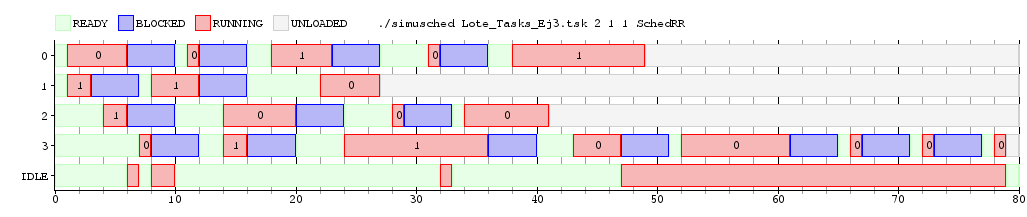
\includegraphics[scale=0.55]{images/Ej3}}
    \caption{FCFS Scheduler con 4 tareas Batch.}
\end{figure}

